%%%%%%%%%%%%%%%%%%%%%%%%%%%%%%%%%%%%%%%%%%%%%%%%%%%%%%%%%%%%%%%%%%%%%%%%
\section{Introduction}
% 1. neutron distribution
% 2. symmetry energy dependence on density

%%%%%%%%%%%%%%%%%%%%%%%%%%%%%%%%%%%%%%%%%%%%%%%%
\subsection{symmetry Energy} 
% what's symmetry energy
% why it is important
% how to know/measure it -- theoritically and experimentally
It has long been a hot topic for nuclear scientists to study how the asymmetry 
between number of proton and nucleon will affect nuclei, especially the binding
energy, which hints us the limit of new isotope elements. Using the simplest 
Liquid Drop Model (LDM), we will get the Bethe-Weizsacker Semi-empirical Mass Foumula:
\begin{equation}
    \label{eq:mass-foumula}
    \begin{gathered}
	E\ (MeV) = \textcolor{black}{a_V A} - \textcolor{blue}{a_S A^{2/3}} - \textcolor{green}{a_C\frac{Z(Z-1)}{A^{1/3}}} - \textcolor{red}{a_A\frac{(N-Z)^2}{A}} + \textcolor{cyan}{\delta(A, Z)} + \dots \\
	\delta(A, Z) = 
	    \begin{cases}
		+\delta_0	& \text{Z, N even} \\
		0		& \text{A odd}	\\
		-\delta_0	& \text{Z, N odd (A even)} \\
	    \end{cases}
    \end{gathered}
\end{equation}

\begin{itemize}
    \color{black} \item Volume term: nucleons attract nearest neighbors 
	through strong force ($a_V \sim 16\ MeV$)
    \color{blue}  \item Surface term: correction to the volume term -- nucleons 
	on the surface aren't completely surrounded by other nucleons
    \color{green} \item Coulomb term: electromagnetic (EM) charge repulsion
    \color{red}   \item Asymmetry term: Pauli exclusion principle
    \color{cyan}  \item Pairing term: spin coupling effect -- if N and Z are even,
	then the nuclei will be stable thanks to the occurance of 'paired spin';
	on the other hand, nuclei with odd number of proton and neutron are usually
	unstable. ($\delta_0 \sim 1\ MeV$, slowly decreasing with A)
\end{itemize}

The first 3 terms are natural and easy to understand, while the 4th term is 
not so obvious. It is based only on Pauli exclusion principle. In heavy nuclei,
more neutrons than protons are needed to balance the repulsion between protons.
Due to the Pauli exclusion principle, these extra neutrons' energy will be 
higher than the rest of nucleons, therefore introducing this correction term.

Regard the nuclear system as a free Fermi gas of protons and neutrons, then the 
kinematic energy of this system will be:
$$ E_k = E_N + E_Z = \frac{3}{5}ZE_F^p + \frac{3}{5}NE_F^n $$
Since the Fermi energy is proportional the $n^{2/3}$
$$ E_k = C(Z^{5/3} + N^{5/3})  $$
Expanse it in terms of N-Z, we will get
\begin{equation*}
    \begin{aligned}
	E_k &= 2^{-2/3}C\left(A^{5/3} + \frac{5}{9}\frac{(N-Z)^2}{A^{1/3}} \right) + O((N-Z)^4) \\
	    &= \frac{3}{5} E_F A + \frac{1}{3}E_F\frac{(N-Z)^2}{A} + O((N-Z)^4) \\
    \end{aligned}
\end{equation*}
The first term contributes to the volume term and the second term is minus the 
asymmetry term because $E_k$ contributes to the binding energy negatively.

For a general discussion, we can ignore the 3rd term to focus on the homogeneous
nuclear (residual strong) interaction between nucleons, and the 5th term which is too small.
Now, we can talk about any nuclear system composed of Z protons (EM charge-less) 
and N neutrons, rather than just true nuclei. Now we have a simplified equation
of state (EoS) for nuclear matter:
\begin{equation}
    \label{eq:modified-mass-formula-1}
    \begin{aligned}
	E &= a_V A - a_S A^{2/3} - a_A\frac{(N-Z)^2}{A}  \\
	e &= \frac{E}{A} = a_V - a_S A^{-1/3} - a_A\frac{(N-Z)^2}{A^2}
    \end{aligned}
\end{equation}

Actually, we should also discard the second term. Obviously, we can't guarantee
any specific shape about the nuclear system; what's mroe, for what people model
with most -- the infinite nuclear system, we don't need to consider the surface 
term at all.
\begin{equation}
    \label{eq:modified-mass-formula-2}
    \begin{aligned}
	E &= a_V A - a_A\frac{(N-Z)^2}{A}  \\
	e &= \frac{E}{A} = a_V - a_A\frac{(N-Z)^2}{A^2} = e_0(A) - a_A\beta^2 
    \end{aligned}
\end{equation}
Here we define $\beta = \frac{N-Z}{A}$ as asymmetry between the number of protons and neutrons. 

For infinite system, density, instead of A, will be a better choice to parameterize
the EoS. So we should replace N, Z and A with their corresponding density: $\rho_n$, 
$\rho_p$ and $\rho$ ($\beta = \frac{\rho_n - \rho_p}{\rho}$). 
So we are considering a infinite uniform nuclear system at 0 temperature that interacts
only via the nuclear force. For any identified $\rho$,
eq \eqref{eq:modified-mass-formula-2} will be:
\begin{equation}
    \label{eq:symmetry-energy}
    e(\rho, \beta) = e(\rho, 0) + S(\rho)\beta^2 + O(\beta^4)
\end{equation}

We find that eq \eqref{eq:modified-mass-formula-2} is a expansion of the 
binding energy per nucleon around $\beta = 0$.
Due to the isospin symmetry between proton and neutron, any isoscalar quantities
F will keep unchanged under $n \leftrightarrow p$ interchange, while isovector 
% change all n into p and p into n. Not just one proton and one neutron
quantities G will change sign. $\beta$ is an isovector, so for a smooth $F(\beta)$,
its expansion around $\beta = 0$ has even terms only:
$$ F(\beta) = F_0 + F_2\beta^2 + F_4\beta^4 + \dots $$
On the other hand, for a smooth $G(\beta)$, its expansion around $\beta = 0$ has
odd terms only:
$$ G(\beta) = G_1\beta + G_3\beta^3 + \dots $$

e is an isoscalar, it doesn't change under $n \leftrightarrow p$ interchange 
as we can see from eq \eqref{eq:modified-mass-formula-2}. The coefficient 
$S(\rho) = \frac{\partial^2 e (\rho, \beta)}{\partial \beta^2}$ is
what we call the \textbf{symmetry energy}, a key parameter in explaining a wide
range of nuclear properties and phenomena. It describes how much energy will be
released when exchange all protons into neutrons for a symmetric nuclear system. 

Not only is $S$ itself important, but also its dependence on $\rho$. 
By convention, $S(\rho)$ is expanded around the nuclear saturation density $\rho_0$
(following the free Fermi gas assumption):
\begin{equation}
    S(\rho) = S(\rho_0) 
    + \left.\frac{dS}{d\rho}\right|_{\rho_0}(\rho - \rho_0)
    + \frac{1}{2}\left.\frac{d^2S}{d\rho^2}\right|_{\rho_0}(\rho - \rho_0)^2
    + \frac{1}{6}\left.\frac{d^3S}{d\rho^3}\right|_{\rho_0}(\rho - \rho_0)^3
    + \dots
\end{equation}
From which, we have some auxiliary parameters defined:
\begin{equation}
    \begin{aligned}
	S_0 &= S(\rho_0)	\\
	L   &= 3\rho_0\left.\frac{dS}{d\rho}\right|_{\rho_0}	\\
	K_{sym}	&= 9\rho_0^2\left.\frac{d^2S}{d\rho^2}\right|_{\rho_0}	\\
	Q_{sym}	&= 27\rho_0^3\left.\frac{d^3S}{d\rho^3}\right|_{\rho_0}	\\
    \end{aligned}
\end{equation}
Among them, L represents S's dependence on $\rho$.

Take neutron star \ref{Lattimer.2001} as an example, it has most neutrons and a few 
protons, so its $\beta = 1$.
\begin{equation}
    \label{eq:neutron-star}
    \begin{aligned}
	 E = E_0 + S	\\
	 P = \rho^2 \frac{dS}{d\rho} \approx \frac{L\rho^2}{3\rho_0}	\\
	 RP^{-1/4} \approx const    \\
    \end{aligned}
\end{equation}
The amazing thing is that neutron star's pressure dependents on L is proportional
to $R^4$. Once we know the L value, we will know the pressure and therefore the 
radius of a neutron star. (Do all neutron stars have the same $\rho$ and R ???)

Being such an important parameter, a great effort has been done to extract S 
and L. Comparing \eqref{eq:modified-mass-formula-2} and \eqref{eq:symmetry-energy},
we can directly get:
\begin{equation}
    S(\rho) \approx -a_A
% S(\rho) = -a_A + \frac{L}{3}\frac{\rho - \rho_0}{\rho_0}
\end{equation}
But this tells us only the symmetry energy at nuclear density ($1.22 \times 10^{44}\ m^{-3}$),
what about the symmetry energy at other density values? Especially at the nuclear
saturation density ($\sim 1.7 \times 10^{44}\ m^{-3}$)? And what about its density
dependence? Another strategy is the energy density functionals (EDF), which fits
the binding energy throughout the nuclear mass table to find out the best EDF,
then use it to calculate $S(\rho)$. The problem is many EDFs can fit equally well
with the binding energy and even the same S value at $\rho_0$, but have quite 
different L values. If there is a experiment that can identify L value without 
model dependence, then no doubt it will help a lot in understanding the symmetry 
energy and the EoS.

% neutron skin
The method to measure L in lab is to measure the neutron skin thickness of 
neutron rich nuclei. For symmetric nuclei (N = Z), the protons and neutrons are
expected to distribute uniformly. While for neutron-rich nuclei, the extra 
neutrons are pushed out against the surface tension\cite{PRL.85.5296}, therefore
forming a neutron skin. 

Neutron skin and neutron star, though of their 18 orders of magnitude difference 
in size (fm vs km), both are neutron-rich nuclear matter and governed by the 
same physical laws: eq \eqref{eq:neutron-star}. So by measuring the neutron
skin thickness, we can derive P and L values, for the study of neutron stars
and nuclear EoS.

%%%%%%%%%%%%%%%%%%%%%%%%%%%%%%%%%%%%%%%%%%%%%%%%
\subsection{Neutron Radius}
There has been many measurements (!!!FIXME!!!) about the charge form factor of many nuclei,
but rarely any precise measurement of the weak form factor of any nuclei.
The Pb Radius EXperiment-II (PREX-II) and Ca48 Radius EXperiment (CREX) are 
high-precision experiments that measures the tiny asymmetry of polarized electrons
scattered from neutron-rich targets to extract the weak form factor and neutron
skin thickness of those nuclei. 

With the high-polarization electron beam at 
Thomas Jefferson National Accelerator Facility (TJNAF, also known as Jlab), 
we were able to measure the asymmetry precisely. 
The cross section asymmetry comes from the interference between 
the electromagnetic (EM) interaction and the weak interaction. While the EM 
cross section has been studied thoroughly, (!!!FIXME!!!: reference) the asymmetry 
measurement allows us to derive the weak charge distribution and finally the
neutron distribution in a nuclear.

There have been many explorations from different aspects to the neutron skin
thickness: hadronic scattering experiment, coherent pion photoproduction,
measurements of electric dipole polarizabilities and pygmy dipole resonances etc.
Though of their valuable efforts, these experiments are trapped by model 
dependence and other uncertainties.


%%%%%%%%%%%%%%%%%%%%%%%%%%%%%%%%%%%%%%%%%%%%%%%%
\subsection{Asymmetry}
\begin{figure}[h]
    \centering
\feynmandiagram[small, vertical' = a to b]{
    i1 [particle = $e^-$] -- [fermion] a -- [fermion] o1 [particle = $e^-$],
    a -- [photon, edge label={Q}, edge label'=$\gamma$] b,
    i2 [particle = p] -- [fermion] b -- [fermion] o2 [particle = p],
    };
\feynmandiagram[small, vertical' = a to b]{
    i1 [particle = $e^-$] -- [fermion] a -- [fermion] o1 [particle = $e^-$],
    a -- [scalar, edge label={Q}, edge label'=Z] b,
    i2 [particle = p] -- [fermion] b -- [fermion] o2 [particle = p],
    };
\end{figure}

\begin{itemize}
    \item $\gamma$ interacts with only vector current
    \item $Z_0$ interacts with both vector and axial-vector current
\end{itemize}

\begin{equation*}
    \CA_{pv} = \frac{\frac{d\sigma^R}{d\Omega} - \frac{d\sigma^L}{d\Omega}}{\frac{d\sigma^R}{d\Omega} + \frac{d\sigma^L}{d\Omega}} = \frac{|\CM^R|^2 - |\CM^L|^2}{|\CM^R|^2 + |\CM^L|^2}
\end{equation*}
where: $\CM^{R, L} = \CM_{\gamma} + \CM_Z^{R,L}$

\begin{equation*}
    \begin{aligned}
	|\CM^{R,L}|^2 &= |\CM_\gamma|^2 + \CM_\gamma\CM_Z^{R,L*} + \CM_\gamma^*\CM_Z^{R,L} + |\CM^{R,L}|^2	\\
	|\CM^{R}|^2 - |\CM^{L}|^2 &= \CM_\gamma( \CM_Z^{R*} - \CM_Z^{L*} + \CM_Z^{R} - \CM_Z^L) \\
	&\approx 2\CM_\gamma(\CM_Z^R - \CM_Z^L)
    \end{aligned}
\end{equation*}


\begin{equation*}
    \begin{aligned}
	\CA_{pv}\footnotemark &\approx \frac{\CM_Z^R - \CM_Z^L}{\CM_\gamma} \propto \frac{\frac{d\sigma_{\text{weak}}}{d\Omega}}{\frac{d\sigma_{\text{E+M}}}{d\Omega}}	\\
	    &\approx \frac{G_F Q^2}{4\pi\alpha\sqrt{2}} \frac{Q_{wk}}{Z}\frac{F_{wk}(Q^2)}{F_{ch}(Q^2)}
    \end{aligned}
\end{equation*}
\begin{equation*}
    \begin{aligned}
	F_{ch}(q) &= G_{ch}^p(q)F_p(q) + G_{ch}^n(q)F_n(q)  \\
		  &= G_E^p(q)F_p(q) + \frac{N}{Z}G_E^n(q)F_n(q)	\\
	F_{wk}(q) &= G_{wk}^p(q)F_p(q) + G_{wk}^n(q)F_n(q)  \\
		  &= G_E^p(q)\left[ F_n(q) - \frac{Z}{N}(1-4\sin^2\theta_W)F_p(q)\right] - G_E^n(q)\left[ F_n(q)(1-4\sin^2\theta_W) - \frac{Z}{N}F_p(q)\right]
    \end{aligned}
\end{equation*}
Where $G_E^p(q)$ and $G_E^n(q)$ are the EW single nucleon FFs, $\sin^2\theta_W = 0.23$ is the Weinberg angle, $F_p(q)$ and $F_n(q)$ are the FFs of point proton and neutron density dist. Compared with $G_E^p(q)$, the charge FF of the neutron $G_E^n(q)$ can be neglected for small momentum transfer:
\begin{equation*}
    \begin{aligned}
	F_p(q) &= \int d^3r j_0(qr) \rho_p(r)	\\
	F_n(q) &= \int d^3r j_0(qr) \rho_n(r)	\\
	G_{wk}^p &= q_p G_E^p + q_n G_E^n + q_0 G_E^s	\\
	G_{wk}^n &= q_p G_E^p + q_n G_E^n + q_0 G_E^s	\\
    \end{aligned}
\end{equation*}
For weak charges including radiative correction
$$ q_p \approx 0.0712	\qquad q_n = q_0 \approx -0.9877 $$
$$ \frac{F_{wk}(q)}{F_{ch}(q)} \approx \frac{F_n(q)}{F_p(q)}$$
$$ \CA_{pv} = \frac{G_FQ^2}{4\pi\alpha\sqrt{2}}\frac{Q_{wk}}{Z}\left[ \frac{F_n(q)}{F_p(q)} - \frac{Z}{N}(1-4\sin^2\theta_W) \right]$$
where: $F(Q^2) = \int d^3r \frac{sin(Qr)}{Qr}\rho(r)$
\begin{equation*}
    \rho(\vec{r}) = Q^{N}\rho_N(\vec{r}) + Q^{P}\rho_P(\vec{r})
\end{equation*}
In general use model for $\rho(\vec{r})$, example: Wood-Saxon form:
\begin{equation*}
    \rho(r) = \frac{\rho_0}{1 + exp[(r-R)/a]}
\end{equation*}
where R is the radius of the density $\rho(r)$?

\bigskip
When ignoring structure (tree level):
\begin{equation*}
    \CA_{\text{pv}} = \frac{G_F Q^2}{\pi\alpha\sqrt{2}} \left(\sin^2\theta_W + \frac{1}{4}\left[ \frac{N}{Z} - 1 \right] \right)
\end{equation*}
\footnotetext[1]{
    for low $Q^2$:
    \begin{equation*}
	\CA_{pv} = \frac{G_F Q^2}{4\pi\alpha\sqrt{2}} \left[ 1- 4\sin^2\theta_W - \frac{F_n(Q^2)}{F_p(Q^2)} \right]
    \end{equation*}
}

\subsection{Dynamics}
\begin{center}
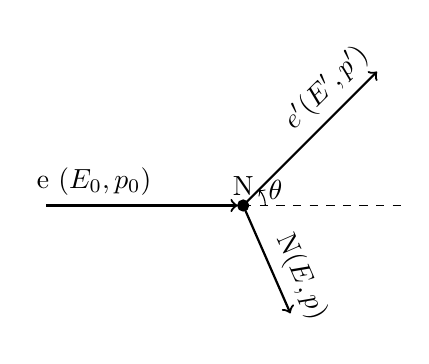
\begin{tikzpicture}
    \coordinate (N) at (0, 0);
    \coordinate (ein) at (-2.5, 0);
    \coordinate (eout) at (1.7, 1.7);
    \coordinate (p) at (0.6, -1.37);

    \filldraw[black] (N) circle (2pt);
    \node [above] at (N) {N};
    \draw[->, thick] (ein) -- node [near start, above] {e ($E_0, p_0$)} ([xshift=-2pt]N);
    \draw[dashed] (N.east) -- +(2, 0);
    \draw[->, thick] (N) -- node[near end, above, sloped] {$e' (E', p')$} (eout);
    \draw[->, thick] (N) -- node[near end, above, sloped] {N($E, p$)} (p);
    \draw [->] ([xshift=8pt]N) arc (0:45:8pt) node[right] {$\theta$};
\end{tikzpicture}
\end{center}

4-Momentum conservation 
$$ E_0 + M = E' + E \qquad \vec{p}_0 = \vec{p}' + \vec{p} $$
Assume ($m_e << 0 \Rightarrow E_0 \approx p_0, E' \approx p'$)
\begin{equation*}
    \begin{aligned}
	E^2 &= M^2 + \vec{p}^2 = M^2 + (\vec{p}_0 - \vec{p}')^2  \\
	    &= M^2 + (E_0 - E'\cos\theta)^2 + (E'\sin\theta)^2	\\
	    &= M^2 + E_0^2 + E'^2 - 2E_0E'\cos\theta	\\
	    &= (E_0 + M - E')^2
    \end{aligned}
\end{equation*}
So we can get
$$ M(E_0 - E') = E_0E'(1-\cos\theta) $$
$$ E' = \frac{ME_0}{M + E_0(1-\cos\theta)}$$
\begin{equation*}
    \begin{aligned}
	Q^2 &= (E_0 - E')^2 - (\vec{p}_0 - \vec{p}')^2	\\
	    &= -2E_0E'(1-\cos\theta)
    \end{aligned}
\end{equation*}

%%%%%%%%%%%%%%%%%%%%%%%%
\subsubsection{Why \Pb and \Ca}
\begin{figure}
    \centering
    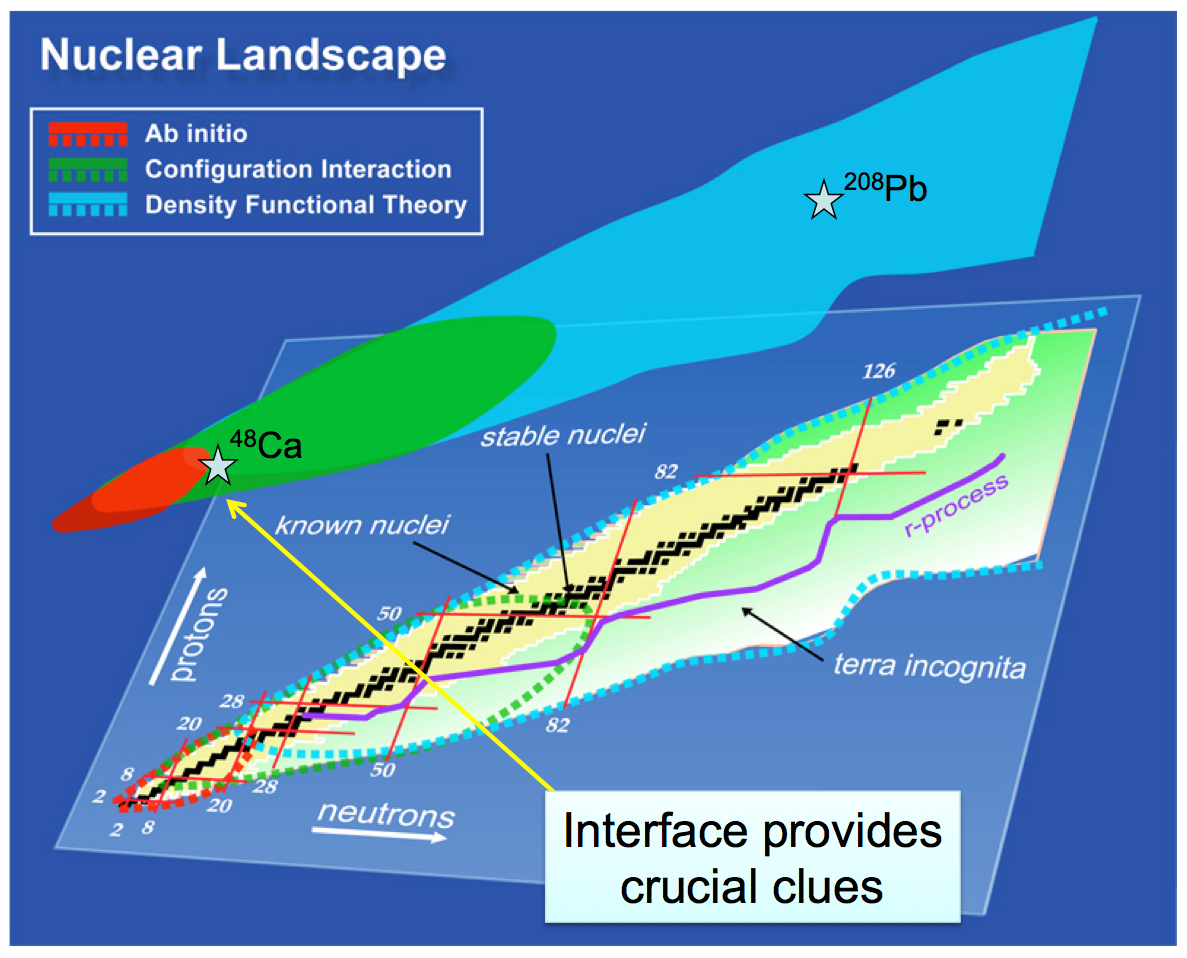
\includegraphics[width=0.5\linewidth]{Nuclear_Landscape}
\end{figure}
